
\chapter{Basics}

\begin{definitionblock}[Algorithm]
    An \textbf{algorithm} is a finite sequence of step-by-step, well-defined instructions that takes some value, or set of values, as input and produces some value, or set of values, as output.
\end{definitionblock}

It can be described by a \textbf{pseudocode}, which can then be converted in any programming language to obtain a working sofftware.

\begin{algorithm}
    \caption{Example: Linear Search}
    \Input{An array $A[1,\dots,n]$ of numbers and a number $q$}
    \Output{An index $i$ such that $A[i] = q$; or \textbf{FAIL} If no such index exists}
    \begin{algorithmic}[1]
        \State $j \gets 1$ \Comment{Variable initialization}
        \While{$j \leq n$} \Comment{Loop syntax, indentation required}
            \If{$A[j] = q$}
                \State \Return $j$ \Comment{Return syntax}
            \EndIf
            \State $j \gets j + 1$
        \EndWhile
        \If{$j = n+1$} \Comment{If syntax, indentation required}
            \State \Return \textbf{FAIL} \Comment{Return syntax}
        \EndIf
    \end{algorithmic}
\end{algorithm}

\begin{definitionblock}[Complexity]
    The \textbf{complexity} of an algorithm is a function that gives the amount of resources (such as time, memory, communication bandwidth, etc.) that the algorithm requires to solve an instance of the problem as a function of the size of the instance.
    In simpler terms, it is the number of "steps" done by the algorithmas a function of the number of input elements.
\end{definitionblock}

We carry on a \textbf{worst-case analysis} of the complexity, which is the maximum number of steps that the algorithm can do for any input. This to guarantee to the user on the performance of the algorithm even with the most unfortunate input. So we want to compute the upper bounds on the running time.

We are interested in the \textbf{order of growth} of an algorithm: the fastest-growing term of the function that expresses the number of steps done by the algorithm in the worst case.

\begin{itemize}
    \item Ignore machine-dependent constants 
    \item Look at the growth of the number of instructions as a function of the input size $n$, when $n \to \infty$
    \item We will express the time complexity of algorithms using the asymptotic notation $O(\cdot)$, $\Omega(\cdot)$, $\Theta(\cdot)$, $o(\cdot)$, $\omega(\cdot)$.
\end{itemize}

\begin{figure}[H]
    \centering
    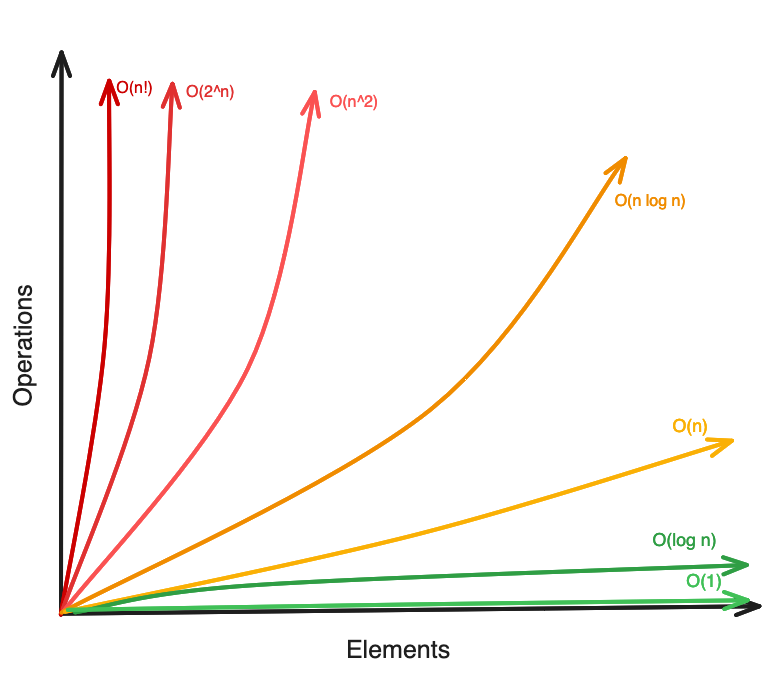
\includegraphics[width=0.7\textwidth]{assets/complexity.png}
    \caption{Complexity}
\end{figure}

\begin{definitionblock}[Time Complexity]
    \begin{itemize}
        \item \textbf{f(n) = O(g(n))} \newline If $\exists c > 0, \hspace{0.2cm}$int$ \hspace{0.1cm} n_0 > 0 \hspace{0.2cm}$s.t. $\hspace{0.2cm} 0 \leq f(n) \leq c\cdot g(n) \hspace{0.2cm} \forall n > n_0$
        \item \textbf{f(n) = o(g(n))} \newline If $\exists c > 0, \hspace{0.2cm}$int$ \hspace{0.1cm} n_0 > 0 \hspace{0.2cm}$s.t. $\hspace{0.2cm} 0 \leq f(n) < c\cdot g(n) \hspace{0.2cm} \forall n > n_0$
        \item \textbf{f(n) = \Omega(g(n))} \newline If $\exists c > 0, \hspace{0.2cm}$int$ \hspace{0.1cm} n_0 > 0 \hspace{0.2cm}$s.t. $\hspace{0.2cm} 0 \leq c\cdot g(n) \leq f(n) \hspace{0.2cm} \forall n > n_0$
        \item \textbf{f(n) = \omega(g(n))} \newline If $\exists c > 0, \hspace{0.2cm}$int$ \hspace{0.1cm} n_0 > 0 \hspace{0.2cm}$s.t. $\hspace{0.2cm} 0 \leq c\cdot g(n) < f(n) \hspace{0.2cm} \forall n > n_0$
        \item \textbf{f(n) = \Theta(g(n))} \newline If $\exists c_1,c_2 > 0, \hspace{0.2cm}$int$ \hspace{0.2cm} n_0 > 0 \hspace{0.2cm}$s.t. $\hspace{0.2cm} 0 \leq c_1\cdot g(n) \leq f(n) \leq c_2\cdot g(n) \hspace{0.2cm} \forall n > n_0$
    \end{itemize}
\end{definitionblock}

We need now to fix a model of computation in order to analyze algorithms. We will start with the most widely used \textbf{RAM Model}.
\begin{itemize}
    \item The model assumes a memory where each cell has a unique address, and accessing any memory cell takes the same constant time, regardless of its location. 
    \item It defines a set of basic operations (e.g., addition, subtraction, comparison, assignment, etc.), each of which is assumed to take constant time.
    \item A single processing unit executes instructions one at a time in a sequential order (no parallelism).
    \item Each word in memory can store a value (e.g., an integer or a pointer), and operations are performed on these words. The model assumes that the size of a word is large enough to hold the required data.
    \item The model abstracts away the low-level details of a real computer, such as cache, paging, or specIfic hardware architecture.
\end{itemize}